\documentclass[12pt, a4paper]{report}
\usepackage[utf8]{inputenc}
\usepackage[T1]{fontenc}
\usepackage{geometry}
\geometry{a4paper, margin=1in, top=1.2in, bottom=1.2in}
\usepackage{graphicx, amsmath, amssymb, booktabs, float, adjustbox, caption, enumitem, titlesec, lmodern}
\usepackage[dvipsnames]{xcolor}
\usepackage{siunitx, pdflscape}
\usepackage[colorlinks=true, linkcolor=black, urlcolor=blue, citecolor=black]{hyperref}
\captionsetup{font=small, labelfont=bf}
\renewcommand{\bibname}{References}
\titleformat{\chapter}[display]{\normalfont\huge\bfseries\raggedright}{\chaptertitlename\ \thechapter}{20pt}{\Huge}
\titlespacing*{\chapter}{0pt}{-20pt}{30pt}
\graphicspath{{fig/}}

\makeatletter
\newcommand{\val}[1]{\@ifundefined{v@#1}{\textcolor{red}{\textbf{??}}}{\csname v@#1\endcsname}}
\makeatother
\expandafter\def\csname v@chk.error\endcsname{0}
\expandafter\def\csname v@chk.info\endcsname{6}
\expandafter\def\csname v@chk.warning\endcsname{1}
\expandafter\def\csname v@chk_overload.error\endcsname{0}
\expandafter\def\csname v@chk_overload.info\endcsname{6}
\expandafter\def\csname v@chk_overload.warning\endcsname{1}
\expandafter\def\csname v@eff.avg\endcsname{97.26}
\expandafter\def\csname v@fault.ilpk\endcsname{12.5}
\expandafter\def\csname v@fault.iout\endcsname{7.63}
\expandafter\def\csname v@fault.rec\endcsname{185}
\expandafter\def\csname v@fault.vout\endcsname{3.81}
\expandafter\def\csname v@fra20.fc\endcsname{3.36}
\expandafter\def\csname v@fra20.pm\endcsname{33}
\expandafter\def\csname v@fra24.fc\endcsname{3.97}
\expandafter\def\csname v@fra24.pm\endcsname{57}
\expandafter\def\csname v@fra36.fc\endcsname{2.93}
\expandafter\def\csname v@fra36.pm\endcsname{70}
\expandafter\def\csname v@fra48.fc\endcsname{3.38}
\expandafter\def\csname v@fra48.pm\endcsname{67}
\expandafter\def\csname v@h24.d\endcsname{0.518}
\expandafter\def\csname v@h24.eff\endcsname{96.81}
\expandafter\def\csname v@h24.effnc\endcsname{96.98}
\expandafter\def\csname v@h24.ilpk\endcsname{8.68}
\expandafter\def\csname v@h24.ilpp\endcsname{2.27}
\expandafter\def\csname v@h24.loss.CIN\endcsname{0.324}
\expandafter\def\csname v@h24.loss.COUT\endcsname{0.003}
\expandafter\def\csname v@h24.loss.L1_core\endcsname{0.159}
\expandafter\def\csname v@h24.loss.L1_dcr\endcsname{1.135}
\expandafter\def\csname v@h24.loss.PCB_Cu\endcsname{0.230}
\expandafter\def\csname v@h24.loss.Q1\endcsname{0.363}
\expandafter\def\csname v@h24.loss.Q2\endcsname{0.087}
\expandafter\def\csname v@h24.loss.Q3\endcsname{0.080}
\expandafter\def\csname v@h24.loss.RS1\endcsname{0.227}
\expandafter\def\csname v@h24.loss.RSN1\endcsname{0.054}
\expandafter\def\csname v@h24.loss.U1_drv_misc\endcsname{0.302}
\expandafter\def\csname v@h24.pin\endcsname{92.76}
\expandafter\def\csname v@h24.pout\endcsname{90.0}
\expandafter\def\csname v@h24.ptot\endcsname{2.96}
\expandafter\def\csname v@h24.rip\endcsname{27.4}
\expandafter\def\csname v@h24.swpk\endcsname{46.6}
\expandafter\def\csname v@h24.vinpp\endcsname{15879}
\expandafter\def\csname v@h24.vout\endcsname{11.997}
\expandafter\def\csname v@h48.d\endcsname{0.257}
\expandafter\def\csname v@h48.eff\endcsname{96.51}
\expandafter\def\csname v@h48.effnc\endcsname{96.80}
\expandafter\def\csname v@h48.ilpk\endcsname{8.98}
\expandafter\def\csname v@h48.ilpp\endcsname{2.93}
\expandafter\def\csname v@h48.loss.CIN\endcsname{0.252}
\expandafter\def\csname v@h48.loss.COUT\endcsname{0.007}
\expandafter\def\csname v@h48.loss.L1_core\endcsname{0.278}
\expandafter\def\csname v@h48.loss.L1_dcr\endcsname{1.143}
\expandafter\def\csname v@h48.loss.PCB_Cu\endcsname{0.202}
\expandafter\def\csname v@h48.loss.Q1\endcsname{0.599}
\expandafter\def\csname v@h48.loss.Q2\endcsname{0.131}
\expandafter\def\csname v@h48.loss.Q3\endcsname{0.041}
\expandafter\def\csname v@h48.loss.RS1\endcsname{0.229}
\expandafter\def\csname v@h48.loss.RSN1\endcsname{0.217}
\expandafter\def\csname v@h48.loss.U1_drv_misc\endcsname{0.156}
\expandafter\def\csname v@h48.pin\endcsname{92.94}
\expandafter\def\csname v@h48.pout\endcsname{90.0}
\expandafter\def\csname v@h48.ptot\endcsname{3.25}
\expandafter\def\csname v@h48.rip\endcsname{32.0}
\expandafter\def\csname v@h48.swpk\endcsname{55.4}
\expandafter\def\csname v@h48.vinpp\endcsname{14741}
\expandafter\def\csname v@h48.vout\endcsname{11.998}
\expandafter\def\csname v@ir.gnd.dv\endcsname{2.3}
\expandafter\def\csname v@ir.gnd.j\endcsname{0.83}
\expandafter\def\csname v@ir.gnd.p\endcsname{12}
\expandafter\def\csname v@ir.gnd.r\endcsname{0.47}
\expandafter\def\csname v@ir.sw.dv\endcsname{5.3}
\expandafter\def\csname v@ir.sw.j\endcsname{2.10}
\expandafter\def\csname v@ir.sw.p\endcsname{27}
\expandafter\def\csname v@ir.sw.r\endcsname{1.06}
\expandafter\def\csname v@ir.vin.dv\endcsname{2.1}
\expandafter\def\csname v@ir.vin.j\endcsname{0.47}
\expandafter\def\csname v@ir.vin.p\endcsname{5}
\expandafter\def\csname v@ir.vin.r\endcsname{0.81}
\expandafter\def\csname v@ir.vout.dv\endcsname{3.3}
\expandafter\def\csname v@ir.vout.j\endcsname{0.68}
\expandafter\def\csname v@ir.vout.p\endcsname{17}
\expandafter\def\csname v@ir.vout.r\endcsname{0.67}
\expandafter\def\csname v@l24_15.d\endcsname{0.504}
\expandafter\def\csname v@l24_15.eff\endcsname{97.21}
\expandafter\def\csname v@l24_15.effnc\endcsname{98.06}
\expandafter\def\csname v@l24_15.ilpk\endcsname{2.30}
\expandafter\def\csname v@l24_15.ilpp\endcsname{2.10}
\expandafter\def\csname v@l24_15.loss.CIN\endcsname{0.013}
\expandafter\def\csname v@l24_15.loss.COUT\endcsname{0.003}
\expandafter\def\csname v@l24_15.loss.L1_core\endcsname{0.134}
\expandafter\def\csname v@l24_15.loss.L1_dcr\endcsname{0.038}
\expandafter\def\csname v@l24_15.loss.PCB_Cu\endcsname{0.008}
\expandafter\def\csname v@l24_15.loss.Q1\endcsname{0.060}
\expandafter\def\csname v@l24_15.loss.Q2\endcsname{0.003}
\expandafter\def\csname v@l24_15.loss.Q3\endcsname{0.013}
\expandafter\def\csname v@l24_15.loss.RS1\endcsname{0.008}
\expandafter\def\csname v@l24_15.loss.RSN1\endcsname{0.054}
\expandafter\def\csname v@l24_15.loss.U1_drv_misc\endcsname{0.097}
\expandafter\def\csname v@l24_15.pin\endcsname{15.29}
\expandafter\def\csname v@l24_15.pout\endcsname{15.0}
\expandafter\def\csname v@l24_15.ptot\endcsname{0.43}
\expandafter\def\csname v@l24_15.vinpp\endcsname{1686}
\expandafter\def\csname v@l24_15.vout\endcsname{11.999}
\expandafter\def\csname v@l24_30.d\endcsname{0.507}
\expandafter\def\csname v@l24_30.eff\endcsname{97.84}
\expandafter\def\csname v@l24_30.effnc\endcsname{98.31}
\expandafter\def\csname v@l24_30.ilpk\endcsname{3.62}
\expandafter\def\csname v@l24_30.ilpp\endcsname{2.19}
\expandafter\def\csname v@l24_30.loss.CIN\endcsname{0.039}
\expandafter\def\csname v@l24_30.loss.COUT\endcsname{0.003}
\expandafter\def\csname v@l24_30.loss.L1_core\endcsname{0.147}
\expandafter\def\csname v@l24_30.loss.L1_dcr\endcsname{0.132}
\expandafter\def\csname v@l24_30.loss.PCB_Cu\endcsname{0.027}
\expandafter\def\csname v@l24_30.loss.Q1\endcsname{0.098}
\expandafter\def\csname v@l24_30.loss.Q2\endcsname{0.012}
\expandafter\def\csname v@l24_30.loss.Q3\endcsname{0.026}
\expandafter\def\csname v@l24_30.loss.RS1\endcsname{0.026}
\expandafter\def\csname v@l24_30.loss.RSN1\endcsname{0.054}
\expandafter\def\csname v@l24_30.loss.U1_drv_misc\endcsname{0.097}
\expandafter\def\csname v@l24_30.pin\endcsname{30.51}
\expandafter\def\csname v@l24_30.pout\endcsname{30.0}
\expandafter\def\csname v@l24_30.ptot\endcsname{0.66}
\expandafter\def\csname v@l24_30.vinpp\endcsname{3823}
\expandafter\def\csname v@l24_30.vout\endcsname{11.999}
\expandafter\def\csname v@l24_6.d\endcsname{0.502}
\expandafter\def\csname v@l24_6.eff\endcsname{94.21}
\expandafter\def\csname v@l24_6.effnc\endcsname{96.41}
\expandafter\def\csname v@l24_6.ilpk\endcsname{1.57}
\expandafter\def\csname v@l24_6.ilpp\endcsname{2.19}
\expandafter\def\csname v@l24_6.loss.CIN\endcsname{0.005}
\expandafter\def\csname v@l24_6.loss.COUT\endcsname{0.003}
\expandafter\def\csname v@l24_6.loss.L1_core\endcsname{0.146}
\expandafter\def\csname v@l24_6.loss.L1_dcr\endcsname{0.011}
\expandafter\def\csname v@l24_6.loss.PCB_Cu\endcsname{0.002}
\expandafter\def\csname v@l24_6.loss.Q1\endcsname{0.031}
\expandafter\def\csname v@l24_6.loss.Q2\endcsname{0.003}
\expandafter\def\csname v@l24_6.loss.Q3\endcsname{0.005}
\expandafter\def\csname v@l24_6.loss.RS1\endcsname{0.002}
\expandafter\def\csname v@l24_6.loss.RSN1\endcsname{0.054}
\expandafter\def\csname v@l24_6.loss.U1_drv_misc\endcsname{0.105}
\expandafter\def\csname v@l24_6.pin\endcsname{6.22}
\expandafter\def\csname v@l24_6.pout\endcsname{6.0}
\expandafter\def\csname v@l24_6.ptot\endcsname{0.37}
\expandafter\def\csname v@l24_6.vinpp\endcsname{1244}
\expandafter\def\csname v@l24_6.vout\endcsname{11.999}
\expandafter\def\csname v@l48_15.d\endcsname{0.252}
\expandafter\def\csname v@l48_15.eff\endcsname{95.02}
\expandafter\def\csname v@l48_15.effnc\endcsname{96.87}
\expandafter\def\csname v@l48_15.ilpk\endcsname{2.80}
\expandafter\def\csname v@l48_15.ilpp\endcsname{3.04}
\expandafter\def\csname v@l48_15.loss.CIN\endcsname{0.011}
\expandafter\def\csname v@l48_15.loss.COUT\endcsname{0.007}
\expandafter\def\csname v@l48_15.loss.L1_core\endcsname{0.302}
\expandafter\def\csname v@l48_15.loss.L1_dcr\endcsname{0.046}
\expandafter\def\csname v@l48_15.loss.PCB_Cu\endcsname{0.008}
\expandafter\def\csname v@l48_15.loss.Q1\endcsname{0.148}
\expandafter\def\csname v@l48_15.loss.Q2\endcsname{0.007}
\expandafter\def\csname v@l48_15.loss.Q3\endcsname{0.006}
\expandafter\def\csname v@l48_15.loss.RS1\endcsname{0.009}
\expandafter\def\csname v@l48_15.loss.RSN1\endcsname{0.217}
\expandafter\def\csname v@l48_15.loss.U1_drv_misc\endcsname{0.025}
\expandafter\def\csname v@l48_15.pin\endcsname{15.48}
\expandafter\def\csname v@l48_15.pout\endcsname{15.0}
\expandafter\def\csname v@l48_15.ptot\endcsname{0.79}
\expandafter\def\csname v@l48_15.vinpp\endcsname{2219}
\expandafter\def\csname v@l48_15.vout\endcsname{11.999}
\expandafter\def\csname v@l48_30.d\endcsname{0.253}
\expandafter\def\csname v@l48_30.eff\endcsname{96.64}
\expandafter\def\csname v@l48_30.effnc\endcsname{97.57}
\expandafter\def\csname v@l48_30.ilpk\endcsname{4.02}
\expandafter\def\csname v@l48_30.ilpp\endcsname{3.01}
\expandafter\def\csname v@l48_30.loss.CIN\endcsname{0.031}
\expandafter\def\csname v@l48_30.loss.COUT\endcsname{0.007}
\expandafter\def\csname v@l48_30.loss.L1_core\endcsname{0.296}
\expandafter\def\csname v@l48_30.loss.L1_dcr\endcsname{0.140}
\expandafter\def\csname v@l48_30.loss.PCB_Cu\endcsname{0.025}
\expandafter\def\csname v@l48_30.loss.Q1\endcsname{0.217}
\expandafter\def\csname v@l48_30.loss.Q2\endcsname{0.015}
\expandafter\def\csname v@l48_30.loss.Q3\endcsname{0.013}
\expandafter\def\csname v@l48_30.loss.RS1\endcsname{0.028}
\expandafter\def\csname v@l48_30.loss.RSN1\endcsname{0.217}
\expandafter\def\csname v@l48_30.loss.U1_drv_misc\endcsname{0.053}
\expandafter\def\csname v@l48_30.pin\endcsname{30.74}
\expandafter\def\csname v@l48_30.pout\endcsname{30.0}
\expandafter\def\csname v@l48_30.ptot\endcsname{1.04}
\expandafter\def\csname v@l48_30.vinpp\endcsname{3586}
\expandafter\def\csname v@l48_30.vout\endcsname{11.999}
\expandafter\def\csname v@l48_6.d\endcsname{0.251}
\expandafter\def\csname v@l48_6.eff\endcsname{89.93}
\expandafter\def\csname v@l48_6.effnc\endcsname{94.19}
\expandafter\def\csname v@l48_6.ilpk\endcsname{2.02}
\expandafter\def\csname v@l48_6.ilpp\endcsname{3.04}
\expandafter\def\csname v@l48_6.loss.CIN\endcsname{0.005}
\expandafter\def\csname v@l48_6.loss.COUT\endcsname{0.007}
\expandafter\def\csname v@l48_6.loss.L1_core\endcsname{0.302}
\expandafter\def\csname v@l48_6.loss.L1_dcr\endcsname{0.019}
\expandafter\def\csname v@l48_6.loss.PCB_Cu\endcsname{0.003}
\expandafter\def\csname v@l48_6.loss.Q1\endcsname{0.077}
\expandafter\def\csname v@l48_6.loss.Q2\endcsname{0.021}
\expandafter\def\csname v@l48_6.loss.Q3\endcsname{0.003}
\expandafter\def\csname v@l48_6.loss.RS1\endcsname{0.004}
\expandafter\def\csname v@l48_6.loss.RSN1\endcsname{0.217}
\expandafter\def\csname v@l48_6.loss.U1_drv_misc\endcsname{0.013}
\expandafter\def\csname v@l48_6.pin\endcsname{6.37}
\expandafter\def\csname v@l48_6.pout\endcsname{6.0}
\expandafter\def\csname v@l48_6.ptot\endcsname{0.67}
\expandafter\def\csname v@l48_6.vinpp\endcsname{1295}
\expandafter\def\csname v@l48_6.vout\endcsname{11.999}
\expandafter\def\csname v@line.down\endcsname{25}
\expandafter\def\csname v@line.up\endcsname{62}
\expandafter\def\csname v@ls.over\endcsname{168}
\expandafter\def\csname v@ls.settle\endcsname{0.17}
\expandafter\def\csname v@ls.under\endcsname{180}
\expandafter\def\csname v@s20.d\endcsname{0.616}
\expandafter\def\csname v@s20.eff\endcsname{97.55}
\expandafter\def\csname v@s20.effnc\endcsname{97.73}
\expandafter\def\csname v@s20.ilpk\endcsname{5.97}
\expandafter\def\csname v@s20.ilpp\endcsname{1.94}
\expandafter\def\csname v@s20.loss.CIN\endcsname{0.138}
\expandafter\def\csname v@s20.loss.COUT\endcsname{0.002}
\expandafter\def\csname v@s20.loss.L1_core\endcsname{0.113}
\expandafter\def\csname v@s20.loss.L1_dcr\endcsname{0.506}
\expandafter\def\csname v@s20.loss.PCB_Cu\endcsname{0.107}
\expandafter\def\csname v@s20.loss.Q1\endcsname{0.195}
\expandafter\def\csname v@s20.loss.Q2\endcsname{0.035}
\expandafter\def\csname v@s20.loss.Q3\endcsname{0.063}
\expandafter\def\csname v@s20.loss.RS1\endcsname{0.101}
\expandafter\def\csname v@s20.loss.RSN1\endcsname{0.038}
\expandafter\def\csname v@s20.loss.U1_drv_misc\endcsname{0.209}
\expandafter\def\csname v@s20.pin\endcsname{61.36}
\expandafter\def\csname v@s20.pout\endcsname{60.0}
\expandafter\def\csname v@s20.ptot\endcsname{1.51}
\expandafter\def\csname v@s20.rip\endcsname{22.4}
\expandafter\def\csname v@s20.swpk\endcsname{33.3}
\expandafter\def\csname v@s20.vinpp\endcsname{10531}
\expandafter\def\csname v@s20.vout\endcsname{11.997}
\expandafter\def\csname v@s24.d\endcsname{0.512}
\expandafter\def\csname v@s24.eff\endcsname{97.38}
\expandafter\def\csname v@s24.effnc\endcsname{97.64}
\expandafter\def\csname v@s24.ilpk\endcsname{6.20}
\expandafter\def\csname v@s24.ilpp\endcsname{2.33}
\expandafter\def\csname v@s24.loss.CIN\endcsname{0.146}
\expandafter\def\csname v@s24.loss.COUT\endcsname{0.003}
\expandafter\def\csname v@s24.loss.L1_core\endcsname{0.168}
\expandafter\def\csname v@s24.loss.L1_dcr\endcsname{0.509}
\expandafter\def\csname v@s24.loss.PCB_Cu\endcsname{0.103}
\expandafter\def\csname v@s24.loss.Q1\endcsname{0.214}
\expandafter\def\csname v@s24.loss.Q2\endcsname{0.042}
\expandafter\def\csname v@s24.loss.Q3\endcsname{0.053}
\expandafter\def\csname v@s24.loss.RS1\endcsname{0.102}
\expandafter\def\csname v@s24.loss.RSN1\endcsname{0.054}
\expandafter\def\csname v@s24.loss.U1_drv_misc\endcsname{0.222}
\expandafter\def\csname v@s24.pin\endcsname{61.43}
\expandafter\def\csname v@s24.pout\endcsname{60.0}
\expandafter\def\csname v@s24.ptot\endcsname{1.61}
\expandafter\def\csname v@s24.rip\endcsname{25.7}
\expandafter\def\csname v@s24.swpk\endcsname{34.4}
\expandafter\def\csname v@s24.vinpp\endcsname{10629}
\expandafter\def\csname v@s24.vout\endcsname{11.998}
\expandafter\def\csname v@s36.d\endcsname{0.340}
\expandafter\def\csname v@s36.eff\endcsname{97.22}
\expandafter\def\csname v@s36.effnc\endcsname{97.60}
\expandafter\def\csname v@s36.ilpk\endcsname{6.39}
\expandafter\def\csname v@s36.ilpp\endcsname{2.75}
\expandafter\def\csname v@s36.loss.CIN\endcsname{0.133}
\expandafter\def\csname v@s36.loss.COUT\endcsname{0.005}
\expandafter\def\csname v@s36.loss.L1_core\endcsname{0.242}
\expandafter\def\csname v@s36.loss.L1_dcr\endcsname{0.513}
\expandafter\def\csname v@s36.loss.PCB_Cu\endcsname{0.095}
\expandafter\def\csname v@s36.loss.Q1\endcsname{0.291}
\expandafter\def\csname v@s36.loss.Q2\endcsname{0.053}
\expandafter\def\csname v@s36.loss.Q3\endcsname{0.035}
\expandafter\def\csname v@s36.loss.RS1\endcsname{0.103}
\expandafter\def\csname v@s36.loss.RSN1\endcsname{0.122}
\expandafter\def\csname v@s36.loss.U1_drv_misc\endcsname{0.121}
\expandafter\def\csname v@s36.pin\endcsname{61.45}
\expandafter\def\csname v@s36.pout\endcsname{60.0}
\expandafter\def\csname v@s36.ptot\endcsname{1.71}
\expandafter\def\csname v@s36.rip\endcsname{31.4}
\expandafter\def\csname v@s36.swpk\endcsname{40.0}
\expandafter\def\csname v@s36.vinpp\endcsname{9810}
\expandafter\def\csname v@s36.vout\endcsname{11.998}
\expandafter\def\csname v@s48.d\endcsname{0.255}
\expandafter\def\csname v@s48.eff\endcsname{96.91}
\expandafter\def\csname v@s48.effnc\endcsname{97.38}
\expandafter\def\csname v@s48.ilpk\endcsname{6.50}
\expandafter\def\csname v@s48.ilpp\endcsname{3.02}
\expandafter\def\csname v@s48.loss.CIN\endcsname{0.114}
\expandafter\def\csname v@s48.loss.COUT\endcsname{0.007}
\expandafter\def\csname v@s48.loss.L1_core\endcsname{0.296}
\expandafter\def\csname v@s48.loss.L1_dcr\endcsname{0.516}
\expandafter\def\csname v@s48.loss.PCB_Cu\endcsname{0.091}
\expandafter\def\csname v@s48.loss.Q1\endcsname{0.391}
\expandafter\def\csname v@s48.loss.Q2\endcsname{0.058}
\expandafter\def\csname v@s48.loss.Q3\endcsname{0.026}
\expandafter\def\csname v@s48.loss.RS1\endcsname{0.103}
\expandafter\def\csname v@s48.loss.RSN1\endcsname{0.217}
\expandafter\def\csname v@s48.loss.U1_drv_misc\endcsname{0.093}
\expandafter\def\csname v@s48.pin\endcsname{61.60}
\expandafter\def\csname v@s48.pout\endcsname{60.0}
\expandafter\def\csname v@s48.ptot\endcsname{1.91}
\expandafter\def\csname v@s48.rip\endcsname{34.2}
\expandafter\def\csname v@s48.swpk\endcsname{48.8}
\expandafter\def\csname v@s48.vinpp\endcsname{9726}
\expandafter\def\csname v@s48.vout\endcsname{11.998}
\expandafter\def\csname v@start24.IL_pk\endcsname{6.9}
\expandafter\def\csname v@start24.Iin_pk\endcsname{3.9}
\expandafter\def\csname v@start24.Vout_over\endcsname{56}
\expandafter\def\csname v@start24.t_reg_ms\endcsname{7.4}
\expandafter\def\csname v@start24.t_rise_ms\endcsname{6.4}
\expandafter\def\csname v@start48.IL_pk\endcsname{7.5}
\expandafter\def\csname v@start48.Iin_pk\endcsname{2.3}
\expandafter\def\csname v@start48.Vout_over\endcsname{64}
\expandafter\def\csname v@start48.t_reg_ms\endcsname{7.4}
\expandafter\def\csname v@start48.t_rise_ms\endcsname{6.4}
\expandafter\def\csname v@th.h24.CINB1.p\endcsname{0.11}
\expandafter\def\csname v@th.h24.CINB1.ss40\endcsname{54.6}
\expandafter\def\csname v@th.h24.CINB1.t300\endcsname{35.1}
\expandafter\def\csname v@th.h24.CINB2.p\endcsname{0.11}
\expandafter\def\csname v@th.h24.CINB2.ss40\endcsname{54.8}
\expandafter\def\csname v@th.h24.CINB2.t300\endcsname{35.2}
\expandafter\def\csname v@th.h24.CINB3.p\endcsname{0.11}
\expandafter\def\csname v@th.h24.COUT1.p\endcsname{0.00}
\expandafter\def\csname v@th.h24.COUT1.ss40\endcsname{52.6}
\expandafter\def\csname v@th.h24.COUT1.t300\endcsname{32.7}
\expandafter\def\csname v@th.h24.COUT2.p\endcsname{0.00}
\expandafter\def\csname v@th.h24.COUT2.ss40\endcsname{51.6}
\expandafter\def\csname v@th.h24.COUT2.t300\endcsname{31.9}
\expandafter\def\csname v@th.h24.J2.ss40\endcsname{48.8}
\expandafter\def\csname v@th.h24.J2.t300\endcsname{29.5}
\expandafter\def\csname v@th.h24.L1.p\endcsname{1.29}
\expandafter\def\csname v@th.h24.L1.ss40\endcsname{76.1}
\expandafter\def\csname v@th.h24.L1.t300\endcsname{56.1}
\expandafter\def\csname v@th.h24.Q1.p\endcsname{0.52}
\expandafter\def\csname v@th.h24.Q1.ss40\endcsname{72.9}
\expandafter\def\csname v@th.h24.Q1.t300\endcsname{54.1}
\expandafter\def\csname v@th.h24.Q2.p\endcsname{0.25}
\expandafter\def\csname v@th.h24.Q2.ss40\endcsname{68.5}
\expandafter\def\csname v@th.h24.Q2.t300\endcsname{49.8}
\expandafter\def\csname v@th.h24.Q3.p\endcsname{0.08}
\expandafter\def\csname v@th.h24.Q3.ss40\endcsname{58.4}
\expandafter\def\csname v@th.h24.Q3.t300\endcsname{40.0}
\expandafter\def\csname v@th.h24.RS1.p\endcsname{0.23}
\expandafter\def\csname v@th.h24.RS1.ss40\endcsname{67.8}
\expandafter\def\csname v@th.h24.RS1.t300\endcsname{48.4}
\expandafter\def\csname v@th.h24.RSN1.p\endcsname{0.05}
\expandafter\def\csname v@th.h24.RSN1.ss40\endcsname{67.8}
\expandafter\def\csname v@th.h24.RSN1.t300\endcsname{48.9}
\expandafter\def\csname v@th.h24.U1.p\endcsname{0.21}
\expandafter\def\csname v@th.h24.U1.ss40\endcsname{65.7}
\expandafter\def\csname v@th.h24.U1.t300\endcsname{47.1}
\expandafter\def\csname v@th.h24.U5.ss40\endcsname{58.0}
\expandafter\def\csname v@th.h24.U5.t300\endcsname{39.5}
\expandafter\def\csname v@th.h24.board300\endcsname{36.7}
\expandafter\def\csname v@th.h24.boardss\endcsname{40.4}
\expandafter\def\csname v@th.h24.ptot\endcsname{2.96}
\expandafter\def\csname v@th.h48.CINB1.p\endcsname{0.08}
\expandafter\def\csname v@th.h48.CINB1.ss40\endcsname{54.0}
\expandafter\def\csname v@th.h48.CINB1.t300\endcsname{34.2}
\expandafter\def\csname v@th.h48.CINB2.p\endcsname{0.08}
\expandafter\def\csname v@th.h48.CINB2.ss40\endcsname{54.3}
\expandafter\def\csname v@th.h48.CINB2.t300\endcsname{34.4}
\expandafter\def\csname v@th.h48.CINB3.p\endcsname{0.08}
\expandafter\def\csname v@th.h48.COUT1.p\endcsname{0.00}
\expandafter\def\csname v@th.h48.COUT1.ss40\endcsname{54.2}
\expandafter\def\csname v@th.h48.COUT1.t300\endcsname{33.7}
\expandafter\def\csname v@th.h48.COUT2.p\endcsname{0.00}
\expandafter\def\csname v@th.h48.COUT2.ss40\endcsname{53.0}
\expandafter\def\csname v@th.h48.COUT2.t300\endcsname{32.8}
\expandafter\def\csname v@th.h48.J2.ss40\endcsname{49.9}
\expandafter\def\csname v@th.h48.J2.t300\endcsname{30.1}
\expandafter\def\csname v@th.h48.L1.p\endcsname{1.42}
\expandafter\def\csname v@th.h48.L1.ss40\endcsname{80.6}
\expandafter\def\csname v@th.h48.L1.t300\endcsname{60.1}
\expandafter\def\csname v@th.h48.Q1.p\endcsname{0.72}
\expandafter\def\csname v@th.h48.Q1.ss40\endcsname{79.7}
\expandafter\def\csname v@th.h48.Q1.t300\endcsname{60.6}
\expandafter\def\csname v@th.h48.Q2.p\endcsname{0.25}
\expandafter\def\csname v@th.h48.Q2.ss40\endcsname{73.2}
\expandafter\def\csname v@th.h48.Q2.t300\endcsname{54.1}
\expandafter\def\csname v@th.h48.Q3.p\endcsname{0.04}
\expandafter\def\csname v@th.h48.Q3.ss40\endcsname{59.5}
\expandafter\def\csname v@th.h48.Q3.t300\endcsname{40.7}
\expandafter\def\csname v@th.h48.RS1.p\endcsname{0.23}
\expandafter\def\csname v@th.h48.RS1.ss40\endcsname{70.9}
\expandafter\def\csname v@th.h48.RS1.t300\endcsname{51.1}
\expandafter\def\csname v@th.h48.RSN1.p\endcsname{0.22}
\expandafter\def\csname v@th.h48.RSN1.ss40\endcsname{77.3}
\expandafter\def\csname v@th.h48.RSN1.t300\endcsname{58.1}
\expandafter\def\csname v@th.h48.U1.p\endcsname{0.11}
\expandafter\def\csname v@th.h48.U1.ss40\endcsname{68.9}
\expandafter\def\csname v@th.h48.U1.t300\endcsname{49.9}
\expandafter\def\csname v@th.h48.U5.ss40\endcsname{59.4}
\expandafter\def\csname v@th.h48.U5.t300\endcsname{40.6}
\expandafter\def\csname v@th.h48.board300\endcsname{38.0}
\expandafter\def\csname v@th.h48.boardss\endcsname{42.0}
\expandafter\def\csname v@th.h48.ptot\endcsname{3.25}
\expandafter\def\csname v@th.s20.CINB1.p\endcsname{0.05}
\expandafter\def\csname v@th.s20.CINB1.ss40\endcsname{47.0}
\expandafter\def\csname v@th.s20.CINB1.t300\endcsname{29.7}
\expandafter\def\csname v@th.s20.CINB2.p\endcsname{0.05}
\expandafter\def\csname v@th.s20.CINB2.ss40\endcsname{47.1}
\expandafter\def\csname v@th.s20.CINB2.t300\endcsname{29.8}
\expandafter\def\csname v@th.s20.CINB3.p\endcsname{0.05}
\expandafter\def\csname v@th.s20.COUT1.p\endcsname{0.00}
\expandafter\def\csname v@th.s20.COUT1.ss40\endcsname{46.3}
\expandafter\def\csname v@th.s20.COUT1.t300\endcsname{28.8}
\expandafter\def\csname v@th.s20.COUT2.p\endcsname{0.00}
\expandafter\def\csname v@th.s20.COUT2.ss40\endcsname{45.8}
\expandafter\def\csname v@th.s20.COUT2.t300\endcsname{28.4}
\expandafter\def\csname v@th.s20.J2.ss40\endcsname{44.4}
\expandafter\def\csname v@th.s20.J2.t300\endcsname{27.3}
\expandafter\def\csname v@th.s20.L1.p\endcsname{0.62}
\expandafter\def\csname v@th.s20.L1.ss40\endcsname{57.8}
\expandafter\def\csname v@th.s20.L1.t300\endcsname{40.3}
\expandafter\def\csname v@th.s20.Q1.p\endcsname{0.28}
\expandafter\def\csname v@th.s20.Q1.ss40\endcsname{57.2}
\expandafter\def\csname v@th.s20.Q1.t300\endcsname{40.4}
\expandafter\def\csname v@th.s20.Q2.p\endcsname{0.12}
\expandafter\def\csname v@th.s20.Q2.ss40\endcsname{54.8}
\expandafter\def\csname v@th.s20.Q2.t300\endcsname{37.9}
\expandafter\def\csname v@th.s20.Q3.p\endcsname{0.06}
\expandafter\def\csname v@th.s20.Q3.ss40\endcsname{50.2}
\expandafter\def\csname v@th.s20.Q3.t300\endcsname{33.5}
\expandafter\def\csname v@th.s20.RS1.p\endcsname{0.10}
\expandafter\def\csname v@th.s20.RS1.ss40\endcsname{53.6}
\expandafter\def\csname v@th.s20.RS1.t300\endcsname{36.5}
\expandafter\def\csname v@th.s20.RSN1.p\endcsname{0.04}
\expandafter\def\csname v@th.s20.RSN1.ss40\endcsname{54.4}
\expandafter\def\csname v@th.s20.RSN1.t300\endcsname{37.5}
\expandafter\def\csname v@th.s20.U1.p\endcsname{0.15}
\expandafter\def\csname v@th.s20.U1.ss40\endcsname{53.7}
\expandafter\def\csname v@th.s20.U1.t300\endcsname{36.9}
\expandafter\def\csname v@th.s20.U5.ss40\endcsname{49.7}
\expandafter\def\csname v@th.s20.U5.t300\endcsname{33.0}
\expandafter\def\csname v@th.s20.board300\endcsname{31.1}
\expandafter\def\csname v@th.s20.boardss\endcsname{32.9}
\expandafter\def\csname v@th.s20.ptot\endcsname{1.51}
\expandafter\def\csname v@th.s24.CINB1.p\endcsname{0.05}
\expandafter\def\csname v@th.s24.CINB1.ss40\endcsname{47.5}
\expandafter\def\csname v@th.s24.CINB1.t300\endcsname{30.0}
\expandafter\def\csname v@th.s24.CINB2.p\endcsname{0.05}
\expandafter\def\csname v@th.s24.CINB2.ss40\endcsname{47.6}
\expandafter\def\csname v@th.s24.CINB2.t300\endcsname{30.1}
\expandafter\def\csname v@th.s24.CINB3.p\endcsname{0.05}
\expandafter\def\csname v@th.s24.COUT1.p\endcsname{0.00}
\expandafter\def\csname v@th.s24.COUT1.ss40\endcsname{46.8}
\expandafter\def\csname v@th.s24.COUT1.t300\endcsname{29.1}
\expandafter\def\csname v@th.s24.COUT2.p\endcsname{0.00}
\expandafter\def\csname v@th.s24.COUT2.ss40\endcsname{46.2}
\expandafter\def\csname v@th.s24.COUT2.t300\endcsname{28.7}
\expandafter\def\csname v@th.s24.J2.ss40\endcsname{44.8}
\expandafter\def\csname v@th.s24.J2.t300\endcsname{27.4}
\expandafter\def\csname v@th.s24.L1.p\endcsname{0.68}
\expandafter\def\csname v@th.s24.L1.ss40\endcsname{59.3}
\expandafter\def\csname v@th.s24.L1.t300\endcsname{41.6}
\expandafter\def\csname v@th.s24.Q1.p\endcsname{0.30}
\expandafter\def\csname v@th.s24.Q1.ss40\endcsname{58.5}
\expandafter\def\csname v@th.s24.Q1.t300\endcsname{41.5}
\expandafter\def\csname v@th.s24.Q2.p\endcsname{0.13}
\expandafter\def\csname v@th.s24.Q2.ss40\endcsname{55.9}
\expandafter\def\csname v@th.s24.Q2.t300\endcsname{38.8}
\expandafter\def\csname v@th.s24.Q3.p\endcsname{0.05}
\expandafter\def\csname v@th.s24.Q3.ss40\endcsname{50.6}
\expandafter\def\csname v@th.s24.Q3.t300\endcsname{33.8}
\expandafter\def\csname v@th.s24.RS1.p\endcsname{0.10}
\expandafter\def\csname v@th.s24.RS1.ss40\endcsname{54.6}
\expandafter\def\csname v@th.s24.RS1.t300\endcsname{37.3}
\expandafter\def\csname v@th.s24.RSN1.p\endcsname{0.05}
\expandafter\def\csname v@th.s24.RSN1.ss40\endcsname{55.8}
\expandafter\def\csname v@th.s24.RSN1.t300\endcsname{38.7}
\expandafter\def\csname v@th.s24.U1.p\endcsname{0.16}
\expandafter\def\csname v@th.s24.U1.ss40\endcsname{54.7}
\expandafter\def\csname v@th.s24.U1.t300\endcsname{37.7}
\expandafter\def\csname v@th.s24.U5.ss40\endcsname{50.3}
\expandafter\def\csname v@th.s24.U5.t300\endcsname{33.4}
\expandafter\def\csname v@th.s24.board300\endcsname{31.5}
\expandafter\def\csname v@th.s24.boardss\endcsname{33.5}
\expandafter\def\csname v@th.s24.ptot\endcsname{1.61}
\expandafter\def\csname v@th.s48.CINB1.p\endcsname{0.04}
\expandafter\def\csname v@th.s48.CINB1.ss40\endcsname{47.6}
\expandafter\def\csname v@th.s48.CINB1.t300\endcsname{29.9}
\expandafter\def\csname v@th.s48.CINB2.p\endcsname{0.04}
\expandafter\def\csname v@th.s48.CINB2.ss40\endcsname{47.8}
\expandafter\def\csname v@th.s48.CINB2.t300\endcsname{30.0}
\expandafter\def\csname v@th.s48.CINB3.p\endcsname{0.04}
\expandafter\def\csname v@th.s48.COUT1.p\endcsname{0.00}
\expandafter\def\csname v@th.s48.COUT1.ss40\endcsname{48.3}
\expandafter\def\csname v@th.s48.COUT1.t300\endcsname{30.1}
\expandafter\def\csname v@th.s48.COUT2.p\endcsname{0.00}
\expandafter\def\csname v@th.s48.COUT2.ss40\endcsname{47.6}
\expandafter\def\csname v@th.s48.COUT2.t300\endcsname{29.6}
\expandafter\def\csname v@th.s48.J2.ss40\endcsname{45.8}
\expandafter\def\csname v@th.s48.J2.t300\endcsname{28.0}
\expandafter\def\csname v@th.s48.L1.p\endcsname{0.81}
\expandafter\def\csname v@th.s48.L1.ss40\endcsname{63.8}
\expandafter\def\csname v@th.s48.L1.t300\endcsname{45.6}
\expandafter\def\csname v@th.s48.Q1.p\endcsname{0.45}
\expandafter\def\csname v@th.s48.Q1.ss40\endcsname{64.1}
\expandafter\def\csname v@th.s48.Q1.t300\endcsname{46.7}
\expandafter\def\csname v@th.s48.Q2.p\endcsname{0.12}
\expandafter\def\csname v@th.s48.Q2.ss40\endcsname{60.2}
\expandafter\def\csname v@th.s48.Q2.t300\endcsname{42.8}
\expandafter\def\csname v@th.s48.Q3.p\endcsname{0.03}
\expandafter\def\csname v@th.s48.Q3.ss40\endcsname{51.8}
\expandafter\def\csname v@th.s48.Q3.t300\endcsname{34.6}
\expandafter\def\csname v@th.s48.RS1.p\endcsname{0.10}
\expandafter\def\csname v@th.s48.RS1.ss40\endcsname{57.6}
\expandafter\def\csname v@th.s48.RS1.t300\endcsname{39.8}
\expandafter\def\csname v@th.s48.RSN1.p\endcsname{0.22}
\expandafter\def\csname v@th.s48.RSN1.ss40\endcsname{66.9}
\expandafter\def\csname v@th.s48.RSN1.t300\endcsname{49.4}
\expandafter\def\csname v@th.s48.U1.p\endcsname{0.06}
\expandafter\def\csname v@th.s48.U1.ss40\endcsname{57.5}
\expandafter\def\csname v@th.s48.U1.t300\endcsname{40.1}
\expandafter\def\csname v@th.s48.U5.ss40\endcsname{51.7}
\expandafter\def\csname v@th.s48.U5.t300\endcsname{34.5}
\expandafter\def\csname v@th.s48.board300\endcsname{32.7}
\expandafter\def\csname v@th.s48.boardss\endcsname{35.1}
\expandafter\def\csname v@th.s48.ptot\endcsname{1.91}

\newcommand{\simfigure}[4][\textwidth]{\begin{figure}[H]\centering
  \includegraphics[width=#1, height=0.32\textheight, keepaspectratio]{#2}\caption{#3}\label{#4}\end{figure}}
\newcommand{\tallfigure}[4][\textwidth]{\begin{figure}[H]\centering
  \includegraphics[width=#1, height=0.38\textheight, keepaspectratio]{#2}\caption{#3}\label{#4}\end{figure}}
% one row of the component temperature table: ref, name, limit
\newcommand{\throw}[3]{#2 & #3 & \val{th.s24.#1.t300} & \val{th.h48.#1.t300} & \val{th.h48.#1.ss40}\\}

\begin{document}

% ---------------------------------------------------------------- title
\begin{titlepage}
\centering
{\large EE463 Static Power Conversion I\par}
\vspace{1cm}

\includegraphics[width=0.3\textwidth]{logo.png}\par\vspace{1cm}
{\LARGE\bfseries Hardware Project Report\par}
\vspace{0.4cm}
{\Large 60 W, 20--48 V to 12 V Synchronous Buck Converter\par}
\vspace{1.5cm}
{\large Team CMPS\par}
\vspace{0.5cm}
\begin{tabular}{ll}
Yiğit Emre Demiral & 2627792 \\
Vedat Tunahan Ceylan & 2627602 \\
Yasin Baytemir & 2627503 \\
\end{tabular}
\vfill
{\large Middle East Technical University\\ Department of Electrical and Electronics Engineering\par}
\vspace{0.5cm}
{\large \today\par}
\end{titlepage}

\tableofcontents

% ---------------------------------------------------------------- intro
\chapter{Introduction}

The board converts 20--48~V to 12~V at 5~A (60~W) with closed-loop control, and also carries 7.5~A (90~W) for the overload bonus. It is a synchronous buck with the LTC3895 peak current-mode controller, an external average current limit, an ideal-diode input stage for reverse polarity, and a 4-layer \(90\times65\)~mm PCB. Chapter~\ref{ch:design} gives the design and the component choices. Chapter~\ref{ch:circuit} gives the circuit simulations: steady state at all input voltages, switching edges, efficiency and losses, start-up, load and line steps, overload and loop gain. Chapter~\ref{ch:pcb} covers the layout, the course PCB checker and the current flow in the copper. Chapter~\ref{ch:thermal} gives the temperatures for five minutes of continuous operation and for steady state.

All circuit results come from the full switching model with the vendor models of the controller, op amps and MOSFETs, plus estimated parasitics (hot loop 5~nH with snubber, gate loops, traces, capacitor ESR/ESL, 0.5--1~\textmu H supply cable). Steady-state values are taken over the last 2~ms of a 14~ms run. Temperatures come from a finite-volume model of the real board copper with the losses from the circuit simulation.

% ---------------------------------------------------------------- design
\chapter{Design}\label{ch:design}

\section{Specification and Targets}

\begin{table}[H]\centering\caption{Specification and Design Targets}\label{tab:spec}\small
\begin{tabular}{lll}\toprule
Item & Requirement & Design target \\\midrule
Input & 20--48 V DC & on at 16.8 V (RUN), off at 58 V (OVLO) \\
Output & 12 V, 5 A, resistive & same, plus 7.5 A (90 W) \\
Regulation & \(\pm\)2 \% & \(<\pm\)0.5 \% \\
Output ripple & \(\le\)120 mV\(_\text{pp}\) & \(<\)60 mV\(_\text{pp}\) \\
Control & closed loop & peak current mode, analog \\
Auxiliary supplies & from the input only & INTVCC from VIN, then from VOUT \\
Bonus & & 90 W, current limit, reverse polarity, efficiency \\\bottomrule
\end{tabular}\end{table}

The input is always above the output, so a step-down stage is enough and no isolation is needed (Table~\ref{tab:spec}). A synchronous buck has the lowest switch stress (\(V_{DS}=V_{IN}\)) and a continuous output current. At 48~V the low side conducts 75~\% of the time; a 2.6~m\(\Omega\) MOSFET loses about 0.08~W there, a Schottky diode about 1.9~W. This is the largest single step towards the efficiency bonus.

\section{Controller and Current Limit}

The LTC3895 \cite{ltc3895} runs from 4 to 140~V, has a 10~V gate driver, internal bootstrap switch, adaptive dead time and a cycle-by-cycle peak limit. At start-up INTVCC and DRVCC come from VIN; above about 7.7~V output, EXTVCC takes them from the 12~V output, which saves about 0.5~W at 48~V. No external supply is used.

Current mode makes the power stage look like a current source into the output capacitor, so a Type-II network on ITH (8.2~k\(\Omega\), 27~nF, 470~pF) is enough and the loop changes little over the input range. The peak limit of the controller (10.75--14.25~A) is too loose for 7.5~A, so an average limit is added: LT6105 \cite{lt6105} across the 4~m\(\Omega\) shunt (80~mV/A), LT6654 reference \cite{lt6654} and an LT1636 integrator \cite{lt1636} that pulls ITH down through a diode:
\[
I_{lim}=\frac{1.25\cdot 12/23.8}{20\cdot 4\,\text{m}\Omega}=7.88\ \text{A}.
\]

\section{Power Stage}

The duty cycle is 0.60 at 20~V and 0.25 at 48~V. The switching frequency is 94.3~kHz: a 145~kHz version had 2.3~W switching loss in Q1 at 48~V/90~W, and below 90~kHz the inductor ripple at 48~V passes 3~A. The inductor follows from the ripple target of 35~\% of 7.5~A at 48~V:
\[
L=\frac{V_{OUT}(1-D)}{\Delta I_L f_{sw}}=\frac{12\cdot0.75}{0.35\cdot7.5\cdot94.3\,\text{kHz}}\approx 36\ \text{\textmu H}\ \rightarrow\ 33\ \text{\textmu H}.
\]
The XAL1510-333 \cite{xal1510} is shielded, saturates softly and has \(I_{sat}=16.7\)~A, far above the 9~A peak at 90~W.

\begin{table}[H]\centering\caption{Main Power Components}\label{tab:parts}\small
\begin{adjustbox}{max width=\textwidth}
\begin{tabular}{lll}\toprule
Part & Value & Reason \\\midrule
Q1 high side & BSC040N08NS5 \cite{bsc040}, 80 V, 4.0 m\(\Omega\), 43 nC & low gate charge, Q1 loss is mostly switching \\
Q2 low side & BSC026N08NS5 \cite{bsc026}, 80 V, 2.6 m\(\Omega\) & lowest \(R_{DS(on)}\), conducts 40--75 \% \\
Q3 ideal diode & BSC026N08NS5 + LM74700-Q1 \cite{lm74700} & reverse polarity, 20 mV drop \\
L1 & XAL1510-333, 33 \textmu H, 18.7 m\(\Omega\) & shielded, soft saturation \\
C\(_\text{OUT}\) & 2\(\times\)330 \textmu F / 25 V polymer, 16 m\(\Omega\) & low ESR, no DC-bias loss \\
C\(_\text{IN}\) & 10\(\times\)2.2 \textmu F/100 V X7R + 3\(\times\)100 \textmu F/100 V & 3.75 A RMS at 90 W, 24 V \\
Hot loop & 3\(\times\)100 nF/100 V at Q1 drain, 2.2 \(\Omega\) + 1 nF snubber & short loop, damped ringing \\
RS1 & 4 m\(\Omega\), 2 W, 2512 & current limit sense \\\bottomrule
\end{tabular}\end{adjustbox}\end{table}

The output ripple estimate at 48~V is \(\Delta I_L/(8f_{sw}C)+\Delta I_L\,ESR=5.8+23.1=28.9\)~mV\(_\text{pp}\), well inside 120~mV. Table~\ref{tab:parts} lists the main parts. Q1 uses the higher-resistance, lower-charge part on purpose: at \(D=0.25\) its conduction loss is only 0.04~W.

\section{Protection}

Reverse polarity is blocked by Q3 and the LM74700-Q1 (loss about 0.05~W at 24~V/60~W instead of 1--2~W in a diode). RUN and OVLO dividers give 16.8~V turn-on and 58~V turn-off. The average limit holds the output current at 7.88~A; the controller's peak limit and foldback are the backup. A BAT46 clamps negative input transients at the controller.

The full schematic is in Figure~\ref{fig:sch}. All auxiliary ICs run from INTVCC, so the board needs only the main input.

\begin{landscape}\centering
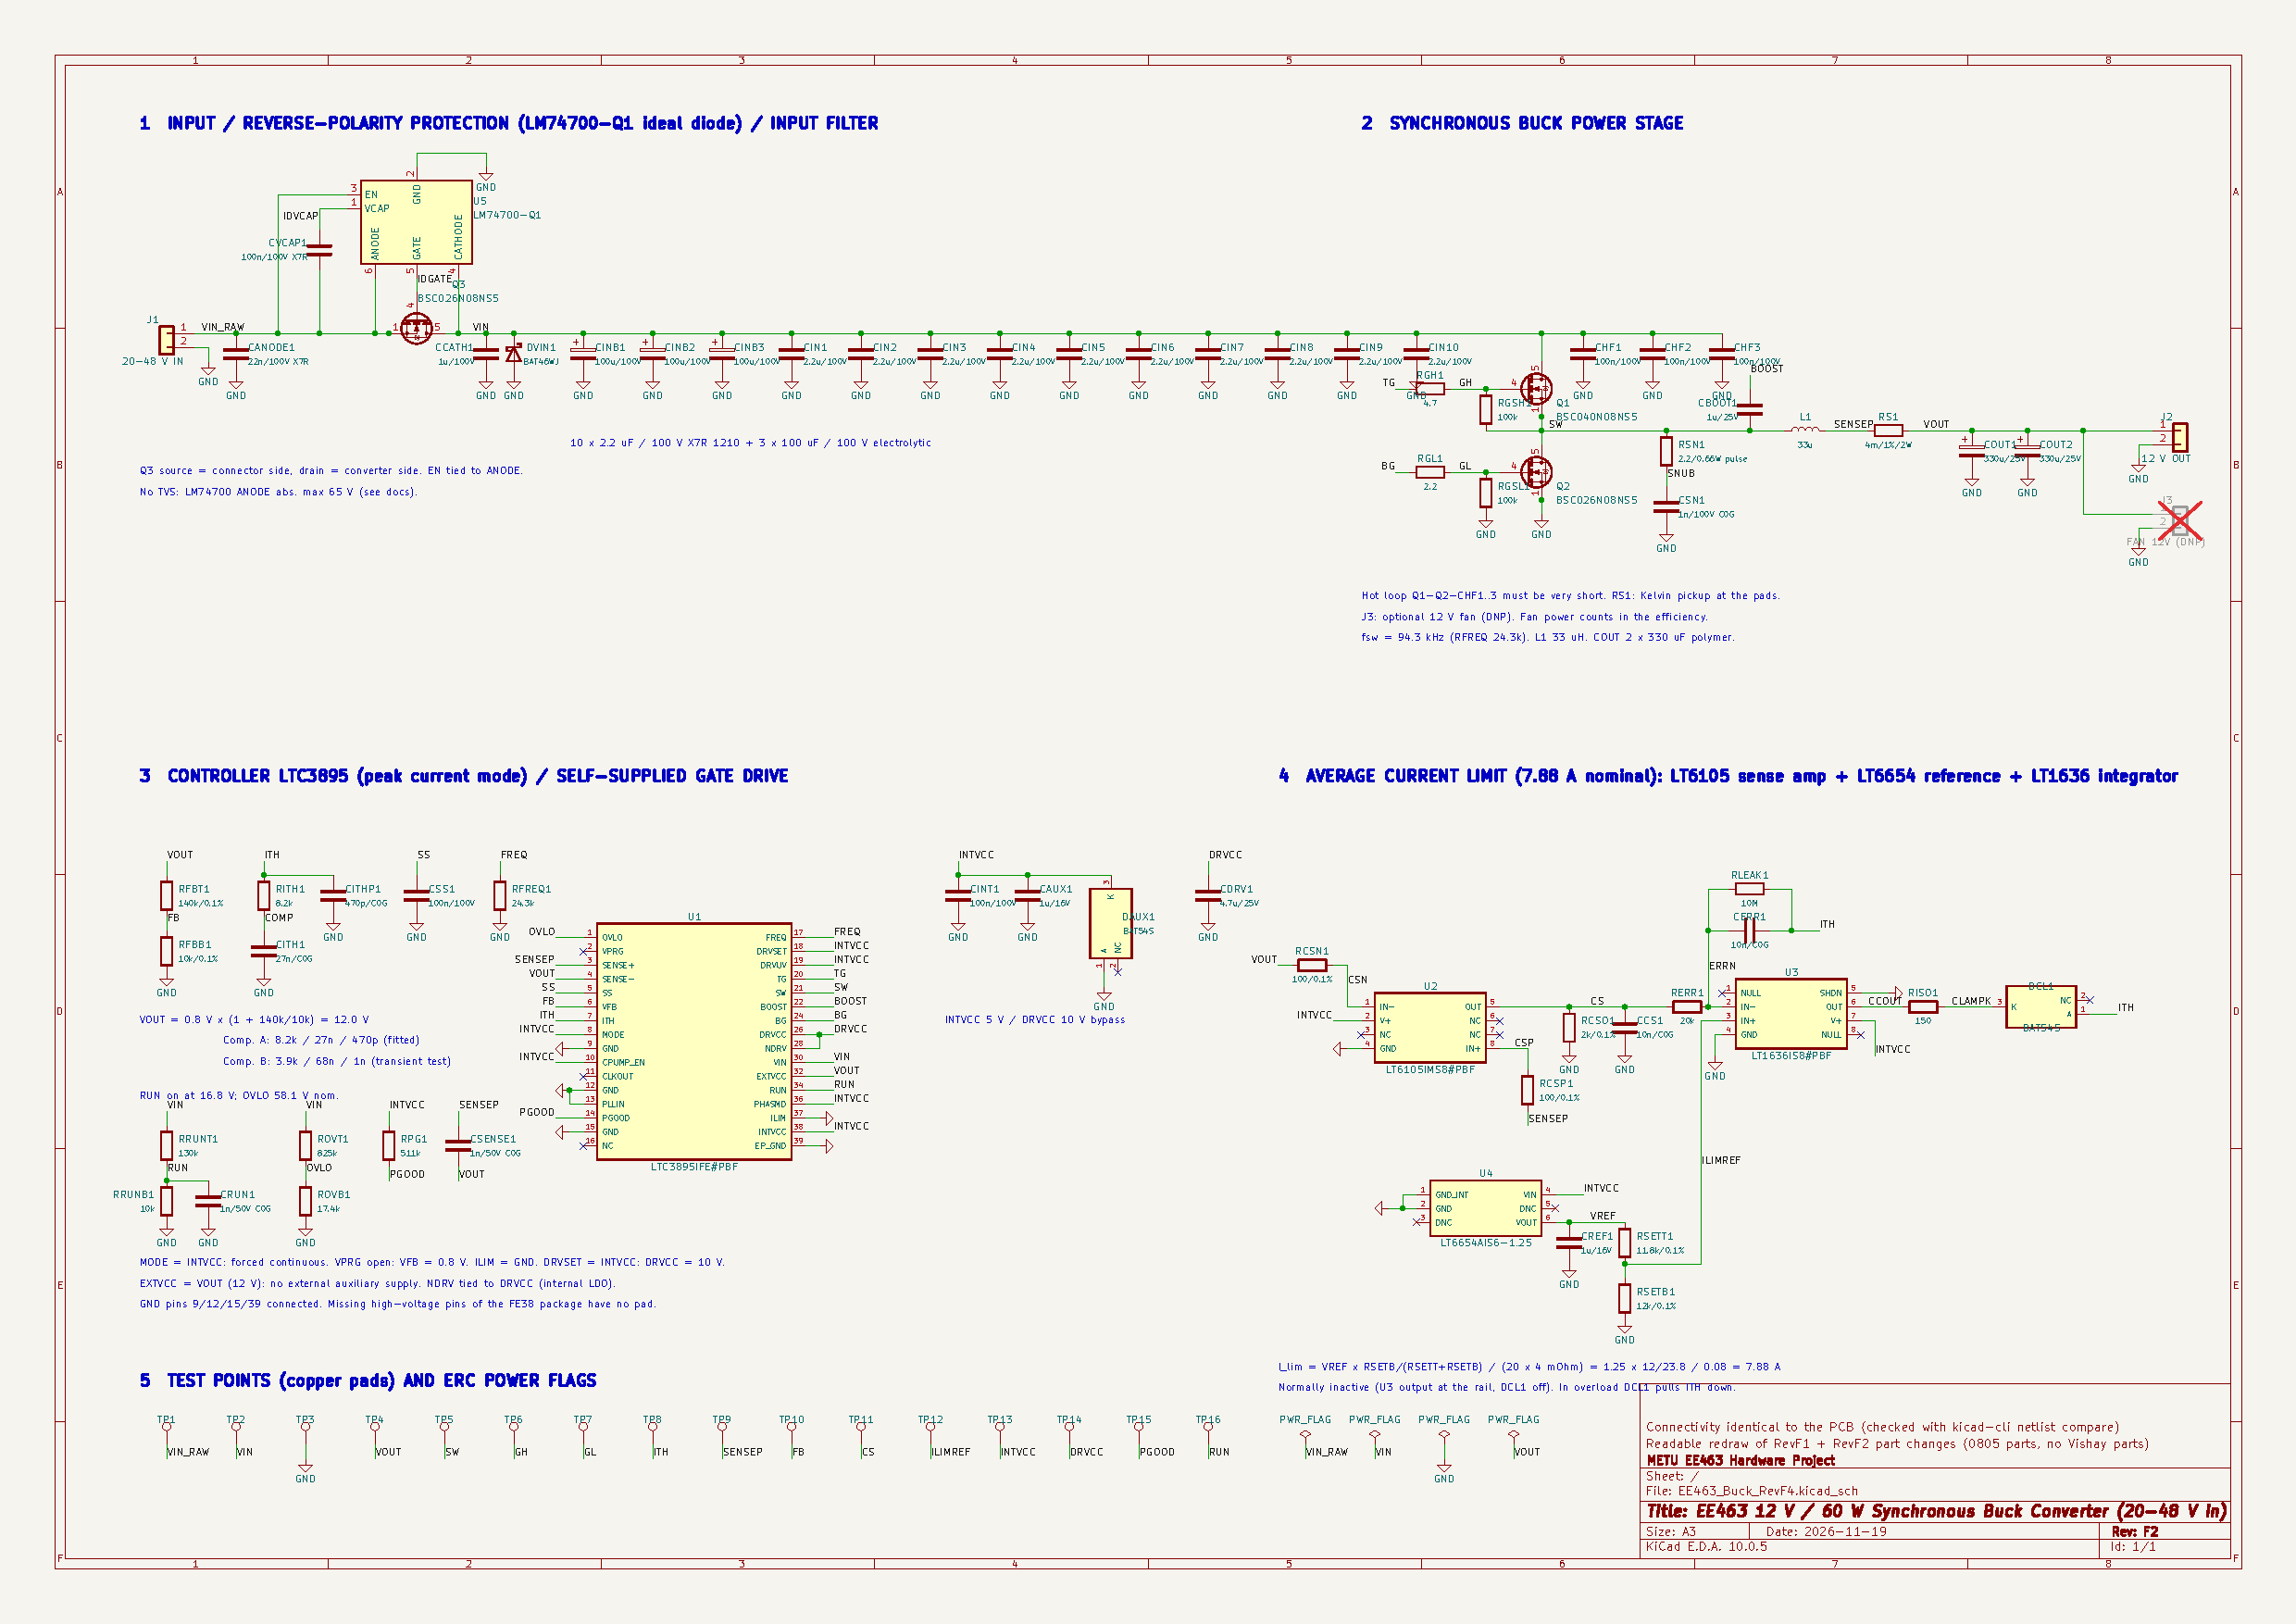
\includegraphics[width=\linewidth, height=0.85\textheight, keepaspectratio]{schematic.pdf}
\captionof{figure}{Schematic, Power Stage and Control}\label{fig:sch}
\end{landscape}

% ---------------------------------------------------------------- circuit
\chapter{Circuit Simulation}\label{ch:circuit}

\section{Steady State}

\begin{table}[H]\centering\caption{Steady-State Results}\label{tab:ss}\small
\begin{adjustbox}{max width=\textwidth}
\begin{tabular}{lcccccc}\toprule
Point & \(V_{OUT}\) [V] & Ripple [mV\(_\text{pp}\)] & \(\Delta I_L\) [A] & \(I_{L,pk}\) [A] & \(V_{SW,pk}\) [V] & \(\eta\) [\%] \\\midrule
20 V / 60 W & \val{s20.vout} & \val{s20.rip} & \val{s20.ilpp} & \val{s20.ilpk} & \val{s20.swpk} & \val{s20.eff} \\
24 V / 60 W & \val{s24.vout} & \val{s24.rip} & \val{s24.ilpp} & \val{s24.ilpk} & \val{s24.swpk} & \val{s24.eff} \\
36 V / 60 W & \val{s36.vout} & \val{s36.rip} & \val{s36.ilpp} & \val{s36.ilpk} & \val{s36.swpk} & \val{s36.eff} \\
48 V / 60 W & \val{s48.vout} & \val{s48.rip} & \val{s48.ilpp} & \val{s48.ilpk} & \val{s48.swpk} & \val{s48.eff} \\
24 V / 90 W & \val{h24.vout} & \val{h24.rip} & \val{h24.ilpp} & \val{h24.ilpk} & \val{h24.swpk} & \val{h24.eff} \\
48 V / 90 W & \val{h48.vout} & \val{h48.rip} & \val{h48.ilpp} & \val{h48.ilpk} & \val{h48.swpk} & \val{h48.eff} \\\bottomrule
\end{tabular}\end{adjustbox}\end{table}

The output stays within 3~mV of 12~V at every point and the ripple is at most a third of the 120~mV limit (Table~\ref{tab:ss}). Efficiency includes the estimated inductor core loss; the average over the four 60~W points is \val{eff.avg}~\%.

\tallfigure{ss_s24.pdf}{Steady-State Waveforms, 24 V, 60 W}{fig:ss24}

Figure~\ref{fig:ss24} shows three switching periods at 24~V. The inductor current is a clean triangle between about 4 and 6~A, the dead time shows as short body-diode steps on the switch node, and the gate voltages reach 10~V.

\tallfigure{ss_s48.pdf}{Steady-State Waveforms, 48 V, 60 W}{fig:ss48}

At 48~V (Figure~\ref{fig:ss48}) the duty cycle drops to \val{s48.d} and the ripple current grows to \val{s48.ilpp}~A, so the output ripple also grows. It is still \val{s48.rip}~mV\(_\text{pp}\).

\tallfigure{ss_h24.pdf}{Steady-State Waveforms, 24 V, 90 W}{fig:ssh24}

At 90~W (Figure~\ref{fig:ssh24}) the average inductor current is 7.5~A and the peak is \val{h24.ilpk}~A, about half of the saturation current. The limit loop stays inactive and the output is \val{h24.vout}~V.

\section{Switching Edges}

\simfigure{edge_s24.pdf}{Switch-Node Rising Edge, 24 V, 60 W}{fig:edge24}

The rising edge takes about 4~ns (Figure~\ref{fig:edge24}). The overshoot comes from the reverse recovery of Q2 with the 5~nH hot-loop inductance; the switch node peaks at \val{s24.swpk}~V at 24~V.

\simfigure{edge_h24.pdf}{Switch-Node Rising Edge, 24 V, 90 W}{fig:edgeh24}

At 90~W the recovery current is larger and the peak reaches \val{h24.swpk}~V at 24~V and \val{h48.swpk}~V at 48~V (Figure~\ref{fig:edgeh24}). This is 69~\% of the 80~V rating in the worst case, so the margin is fine, but it should be measured on the board. If needed, the snubber capacitor can go from 1~nF to 2.2~nF (snubber loss doubles to about 0.4~W at 48~V).

\simfigure{spec_vout.pdf}{Output Voltage Spectrum, 60 W}{fig:spec}

The output spectrum (Figure~\ref{fig:spec}) is dominated by the 94.3~kHz fundamental and its first harmonics. The harmonics fall off quickly, so the ESL of the polymer capacitors adds no visible high-frequency content.

\section{Efficiency and Losses}

\simfigure{eff.pdf}{Efficiency vs Load and vs Input Voltage}{fig:eff}

Efficiency stays above 96~\% from 30~W to 90~W at both 24 and 48~V (Figure~\ref{fig:eff}); at 15~W it is \val{l24_15.eff}~\% at 24~V and \val{l48_15.eff}~\% at 48~V. At light load the fixed losses (gate drive, controller, snubber) dominate, since the controller runs in forced continuous mode.

\simfigure{loss_bar.pdf}{Loss Breakdown per Operating Point}{fig:loss}

\begin{table}[H]\centering\caption{Loss Breakdown [W]}\label{tab:loss}\small
\begin{adjustbox}{max width=\textwidth}
\begin{tabular}{lcccccc}\toprule
 & 20 V/60 W & 24 V/60 W & 36 V/60 W & 48 V/60 W & 24 V/90 W & 48 V/90 W \\\midrule
Q1 & \val{s20.loss.Q1} & \val{s24.loss.Q1} & \val{s36.loss.Q1} & \val{s48.loss.Q1} & \val{h24.loss.Q1} & \val{h48.loss.Q1} \\
Q2 & \val{s20.loss.Q2} & \val{s24.loss.Q2} & \val{s36.loss.Q2} & \val{s48.loss.Q2} & \val{h24.loss.Q2} & \val{h48.loss.Q2} \\
Q3 & \val{s20.loss.Q3} & \val{s24.loss.Q3} & \val{s36.loss.Q3} & \val{s48.loss.Q3} & \val{h24.loss.Q3} & \val{h48.loss.Q3} \\
L1 copper & \val{s20.loss.L1_dcr} & \val{s24.loss.L1_dcr} & \val{s36.loss.L1_dcr} & \val{s48.loss.L1_dcr} & \val{h24.loss.L1_dcr} & \val{h48.loss.L1_dcr} \\
L1 core (est.) & \val{s20.loss.L1_core} & \val{s24.loss.L1_core} & \val{s36.loss.L1_core} & \val{s48.loss.L1_core} & \val{h24.loss.L1_core} & \val{h48.loss.L1_core} \\
RS1 & \val{s20.loss.RS1} & \val{s24.loss.RS1} & \val{s36.loss.RS1} & \val{s48.loss.RS1} & \val{h24.loss.RS1} & \val{h48.loss.RS1} \\
Snubber & \val{s20.loss.RSN1} & \val{s24.loss.RSN1} & \val{s36.loss.RSN1} & \val{s48.loss.RSN1} & \val{h24.loss.RSN1} & \val{h48.loss.RSN1} \\
Capacitors & \val{s20.loss.CIN} & \val{s24.loss.CIN} & \val{s36.loss.CIN} & \val{s48.loss.CIN} & \val{h24.loss.CIN} & \val{h48.loss.CIN} \\
Driver, IC, other & \val{s20.loss.U1_drv_misc} & \val{s24.loss.U1_drv_misc} & \val{s36.loss.U1_drv_misc} & \val{s48.loss.U1_drv_misc} & \val{h24.loss.U1_drv_misc} & \val{h48.loss.U1_drv_misc} \\\midrule
Total & \val{s20.ptot} & \val{s24.ptot} & \val{s36.ptot} & \val{s48.ptot} & \val{h24.ptot} & \val{h48.ptot} \\\bottomrule
\end{tabular}\end{adjustbox}\end{table}

The inductor is the largest loss at every point (Figure~\ref{fig:loss} and Table~\ref{tab:loss}). Q1 loss grows with input voltage because its switching loss scales with \(V_{IN}\); Q2 stays small since it switches at zero voltage. The core loss is not in the inductor model; it is estimated from the vendor loss curve as \(0.12\,(\Delta I_L/2)^{2.2}\)~W and should be checked with the vendor calculator.

\section{Start-Up}

\simfigure{start24.pdf}{Start-Up at 24 V with 2.4 Ohm Load}{fig:st24}

From a 24~V supply with a current limit, the output rises from 10~\% to 90~\% in \val{start24.t_rise_ms}~ms with \val{start24.Vout_over}~mV overshoot (Figure~\ref{fig:st24}). The input current peaks at \val{start24.Iin_pk}~A while the output capacitors charge, so a lab supply set to 6~A does not limit.

\simfigure{start48.pdf}{Start-Up at 48 V with 2.4 Ohm Load}{fig:st48}

At 48~V (Figure~\ref{fig:st48}) the soft start sets the same rise time, \val{start48.t_rise_ms}~ms, and the input current peak drops to \val{start48.Iin_pk}~A.

\section{Load and Line Steps}

\simfigure{loadstep.pdf}{Load Step 5 A to 2.5 A and Back, 24 V}{fig:ls}

A 50~\% load step gives \val{ls.under}~mV undershoot and \val{ls.over}~mV overshoot, both inside the \(\pm\)240~mV band, and the output is back within 1~\% in \val{ls.settle}~ms (Figure~\ref{fig:ls}). There is no ringing, which matches the phase margin in Section~\ref{sec:loop}.

\simfigure{linestep.pdf}{Line Step 24 V to 36 V to 24 V, 60 W}{fig:line}

A 12~V input step moves the output by only \val{line.up}~mV (Figure~\ref{fig:line}). Current-mode control corrects the inductor current in the same cycle, so the voltage loop sees almost nothing.

\section{Overload and Current Limit}

\simfigure{fault.pdf}{Overload, Load 2.4 Ohm to 0.5 Ohm, 24 V}{fig:fault}

With a 0.5~\(\Omega\) load the average limit holds the output current at \val{fault.iout}~A and the output falls to \val{fault.vout}~V (Figure~\ref{fig:fault}). The design value is 7.88~A, so 7.5~A at 90~W is still regulated. The inductor peak during the transition is \val{fault.ilpk}~A, below saturation. When the load returns to 2.4~\(\Omega\) the output overshoots by \val{fault.rec}~mV for well under a millisecond.

\section{Loop Gain}\label{sec:loop}

\simfigure{bode.pdf}{Loop Gain from the Switching Model, 60 W}{fig:bode}

\begin{table}[H]\centering\caption{Crossover Frequency and Phase Margin}\label{tab:fra}\small
\begin{tabular}{lcccc}\toprule
 & 20 V & 24 V & 36 V & 48 V \\\midrule
\(f_c\) [kHz] & \val{fra20.fc} & \val{fra24.fc} & \val{fra36.fc} & \val{fra48.fc} \\
PM [\(^\circ\)] & \val{fra20.pm} & \val{fra24.pm} & \val{fra36.pm} & \val{fra48.pm} \\\bottomrule
\end{tabular}\end{table}

The loop gain was measured on the switching model by injecting a small signal in series with the feedback divider (Figure~\ref{fig:bode}, Table~\ref{tab:fra}). Crossover is at 3--4~kHz at all inputs, well below \(f_{sw}/10\). The phase margin is 57--70\(^\circ\) from 24 to 48~V. The 20~V curve is noisy below 3~kHz and its single point near crossover gives \val{fra20.pm}\(^\circ\); a longer run on the earlier revision with the same compensation gave 54\(^\circ\) at 20~V, and the load step shows no ringing, so the low value is a measurement artefact. It will be checked on the board. The rise near \(f_{sw}/2\) is aliasing of the sampled current loop, not a real gain margin.

% ---------------------------------------------------------------- pcb
\chapter{PCB Design and Checks}\label{ch:pcb}

\section{Layout}

\simfigure[0.7\textwidth]{pcb3d.png}{3D View of the Board, Top Side}{fig:3d}

The board is 90\(\times\)65~mm, 1.6~mm, 1~oz copper on 4 layers (Figure~\ref{fig:3d}). The power path runs from J1 through Q3, the input capacitors and Q1/Q2 to L1, RS1, the output capacitors and J2, all on the top layer.

\simfigure[0.85\textwidth]{pcb_top.pdf}{Top Copper, Silkscreen and Outline}{fig:top}

Q1, Q2 and the three 100~nF capacitors form a hot loop of about 1~nH right at the top of the board (Figure~\ref{fig:top}). The controller sits next to the MOSFETs, so the gate loops are short. Power tracks keep a constant width along their run, and each large pad with several ground vias is joined to them by a small copper pour instead of separate tracks.

\simfigure[0.75\textwidth]{pcb_bottom.pdf}{Bottom Copper and Silkscreen (Mirrored)}{fig:bot}

The inner layers are a solid ground plane (In1) and the VIN/VOUT pours with inner signals (In2). The bottom layer carries signals and ground, and an exposed VIN copper area under Q1 for an optional heatsink (Figure~\ref{fig:bot}). Feedback and current-sense traces are Kelvin-connected at the shunt and routed away from the switch node.

\section{Course PCB Checker}

The board was run through the course PCB checker at both the 5~A rating and the 7.5~A overload setting. The first run gave one error and five warnings:

\begin{itemize}[nosep]
\item three vias 0.35~mm from the drill of a through-hole input capacitor (minimum 0.41~mm),
\item VOUT and GND changing layer through only four 0.3~mm vias,
\item four open vias inside the pads of the 1206 capacitor at the ideal-diode cathode,
\item a 0.2~mm VOUT sense trace on the bottom layer under L1,
\item four copper layers instead of two.
\end{itemize}

The three vias next to the capacitor drills were removed; the through-hole pads already connect all layers. The in-pad vias were removed, a ground via next to the pad stays. Twelve 0.4~mm vias now sit inside the large RS1 output pad, and eleven 0.4~mm ground vias inside a small pour at the Q2 sources take the ground return to the inner plane; that is 8.4~A and 7.7~A of via capacity. The sense trace under L1 was kept: the inductor is shielded, the solid In1 ground plane lies between them, and the area above L1 is taken by the VIN heatsink copper. It is recorded as a waiver in the checker settings.

\begin{table}[H]\centering\caption{PCB Checker Result After the Fixes}\label{tab:chk}\small
\begin{tabular}{lccc}\toprule
Setting & Must fix & Should fix & To check \\\midrule
5 A rating & \val{chk.error} & \val{chk.warning} & \val{chk.info} \\
7.5 A overload & \val{chk_overload.error} & \val{chk_overload.warning} & \val{chk_overload.info} \\\bottomrule
\end{tabular}\end{table}

The only warning left is the layer count (Table~\ref{tab:chk}); the board needs the inner ground plane for the hot loop and the thermal path, so this will be agreed with the course staff before ordering. The items to check by hand are small silkscreen text, gate loops (the checker cannot trace the controller's internal drivers), no thermal vias under the Q2 drain pad (the drain is the switch node, so vias would only add switch-node area), and some 90\(^\circ\) corners on signal traces. KiCad DRC, unconnected items and schematic parity are all zero.

\section{Current Flow in the Copper}

The DC current flow in the four high-current nets was solved on the real copper of all layers on a 0.2~mm grid, with the vias as resistors between layers.

\simfigure{ir_sw.pdf}{Current Density, Switch Node Q1/Q2 to L1, 5 A}{fig:irsw}

The switch node is the narrowest power path. Its resistance is \val{ir.sw.r}~m\(\Omega\) and the highest density is \val{ir.sw.j}~A/mm at the L1 pad entry (Figure~\ref{fig:irsw}). The IPC-2221 limit for 1~oz outer copper and 20~\(^\circ\)C rise is about 3~A/mm, so the copper is adequate.

\simfigure{ir_vout.pdf}{Current Density, VOUT from RS1 to J2, 5 A}{fig:irvout}

The output path shares the current between the top track and the In2 pour (Figure~\ref{fig:irvout}): \val{ir.vout.r}~m\(\Omega\), \val{ir.vout.dv}~mV drop at 5~A.

\simfigure{ir_gnd.pdf}{Current Density, Ground Return, 5 A}{fig:irgnd}

\begin{table}[H]\centering\caption{DC Resistance and Loss of the Power Copper}\label{tab:ir}\small
\begin{tabular}{lcccc}\toprule
Net & \(R\) [m\(\Omega\)] & \(\Delta V\) [mV] & \(P\) [mW] & \(J_{max}\) [A/mm] \\\midrule
SW (5 A) & \val{ir.sw.r} & \val{ir.sw.dv} & \val{ir.sw.p} & \val{ir.sw.j} \\
VOUT (5 A) & \val{ir.vout.r} & \val{ir.vout.dv} & \val{ir.vout.p} & \val{ir.vout.j} \\
GND (5 A) & \val{ir.gnd.r} & \val{ir.gnd.dv} & \val{ir.gnd.p} & \val{ir.gnd.j} \\
VIN (2.6 A, 24 V) & \val{ir.vin.r} & \val{ir.vin.dv} & \val{ir.vin.p} & \val{ir.vin.j} \\\bottomrule
\end{tabular}\end{table}

The ground return spreads over three layers and has the lowest resistance (Figure~\ref{fig:irgnd}, Table~\ref{tab:ir}). The total copper loss in the power paths is under 70~mW, about 0.1~\% of the output power.

% ---------------------------------------------------------------- thermal
\chapter{Thermal Analysis}\label{ch:thermal}

\section{Model}

The board is split into four copper layers and the FR-4 between them on a 0.5~mm grid. Each cell gets the copper fraction of its layer from the board file, the vias add vertical copper, and the top and bottom surfaces lose heat by convection and radiation (\(h=14\) and 10~W/m\(^2\)K). The inductor, the electrolytic and polymer capacitors and the terminals are added as lumped bodies on their pads. Junction temperatures add \(R_{\theta JC}\) times the part loss (Q1 1.2, Q2/Q3 0.9, U1 3~K/W). The losses come from Table~\ref{tab:loss}; the controller and driver residual is split between U1 and the MOSFETs.

\simfigure{copper.pdf}{Copper Distribution of the Four Layers and the Vias}{fig:cu}

Figure~\ref{fig:cu} shows the copper the model uses. The inner ground plane covers almost the whole board, which spreads heat from the MOSFETs and the inductor pads. The board time constant is about 210~s, so five minutes reach about 90~\% of the final temperature rise.

\section{Five Minutes of Continuous Operation}

\simfigure{th_time_s24.pdf}{Temperature vs Time, 24 V, 60 W, 25 C Ambient}{fig:tt24}

At 24~V/60~W the hottest parts are L1 and Q1, both near \val{th.s24.Q1.t300}~\(^\circ\)C after 300~s (Figure~\ref{fig:tt24}). The total loss is \val{th.s24.ptot}~W.

\simfigure{th_time_h48.pdf}{Temperature vs Time, 48 V, 90 W, 25 C Ambient}{fig:tt48}

The worst case is 48~V at 90~W with \val{th.h48.ptot}~W loss (Figure~\ref{fig:tt48}). After five minutes Q1 reaches \val{th.h48.Q1.t300}~\(^\circ\)C and the L1 body \val{th.h48.L1.t300}~\(^\circ\)C. The curves are still rising slowly at 300~s, which is why the steady state is also given below.

\simfigure{th_map_s24.pdf}{Top-Layer Temperature, 24 V, 60 W}{fig:map24}

The heat stays around the power stage in the upper half of the board (Figure~\ref{fig:map24}). The current-limit ICs in the lower half warm up by only about 8--11~\(^\circ\)C even at 90~W.

\simfigure{th_map_h48.pdf}{Top-Layer Temperature, 48 V, 90 W}{fig:map48}

At 90~W the hot spot is between Q1 and L1 (Figure~\ref{fig:map48}). The snubber resistor next to Q2 is also warm at 48~V because its loss scales with \(V_{IN}^2\).

\simfigure{th_layers_h48.pdf}{Temperature of Each Layer at 300 s, 48 V, 90 W}{fig:lay48}

Under the hot spot the bottom layer is about 11~\(^\circ\)C cooler than the top (Figure~\ref{fig:lay48}). The heat spreads mostly in the top copper and the In1 ground plane; the FR-4 between the layers limits the vertical flow, which is why the vias near Q1 and the inductor pads matter.

\simfigure{th_bar.pdf}{Component Temperatures After 5 Minutes, All Operating Points}{fig:thbar}

\begin{table}[H]\centering\caption{Component Temperatures [\(^\circ\)C]}\label{tab:th}\small
\begin{adjustbox}{max width=\textwidth}
\begin{tabular}{lcccc}\toprule
Part & Limit & 24 V/60 W, 300 s, 25 \(^\circ\)C & 48 V/90 W, 300 s, 25 \(^\circ\)C & 48 V/90 W, steady, 40 \(^\circ\)C \\\midrule
\throw{Q1}{Q1 junction}{150}
\throw{Q2}{Q2 junction}{150}
\throw{Q3}{Q3 junction}{150}
\throw{U1}{U1 junction}{125}
\throw{L1}{L1 body}{125}
\throw{RS1}{RS1 shunt}{155}
\throw{RSN1}{RSN1 snubber}{155}
\throw{COUT1}{COUT1 body}{105}
\throw{CINB2}{CINB2 body}{105}
\throw{U5}{U5 LM74700}{125}
\throw{J2}{J2 terminal}{105}
\bottomrule
\end{tabular}\end{adjustbox}\end{table}

Even at 48~V/90~W in steady state at 40~\(^\circ\)C ambient, Q1 reaches \val{th.h48.Q1.ss40}~\(^\circ\)C and L1 \val{th.h48.L1.ss40}~\(^\circ\)C (Figure~\ref{fig:thbar}, Table~\ref{tab:th}). Every part keeps at least 44~\(^\circ\)C margin to its limit, so no heatsink or fan is needed. The electrolytic input capacitors stay close to the board temperature, which matters for their lifetime more than for their rating.

% ---------------------------------------------------------------- conclusion
\chapter{Conclusion}

\textbf{Design.} A synchronous buck with peak current-mode control, an average current limit and an ideal-diode input meets all specifications and the 90~W, current-limit and reverse-polarity bonus targets from one 20--48~V input without any external supply.

\textbf{Circuit.} The output stays within 3~mV of 12~V with at most \val{s48.rip}~mV ripple. Efficiency is \val{s24.eff}~\% at 24~V/60~W and \val{eff.avg}~\% on average over the four input points, including the estimated core loss. A 50~\% load step settles in \val{ls.settle}~ms with \val{ls.under}~mV deviation, and overload is limited at \val{fault.iout}~A. Crossover is 3--4~kHz with 57--70\(^\circ\) phase margin from 24 to 48~V; the 20~V margin and the switch-node peak (\val{h48.swpk}~V at 48~V/90~W) are the two values to measure first on the board.

\textbf{PCB.} The board passes the course PCB checker with no errors at both 5~A and 7.5~A; the only open item is the 4-layer stack-up, which needs approval. The power copper has 0.5--1.1~m\(\Omega\) resistance and less than 70~mW loss.

\textbf{Thermal.} After five minutes at 25~\(^\circ\)C ambient the hottest junction is \val{th.s24.Q1.t300}~\(^\circ\)C at 24~V/60~W and \val{th.h48.Q1.t300}~\(^\circ\)C at 48~V/90~W. In steady state at 40~\(^\circ\)C it is \val{th.h48.Q1.ss40}~\(^\circ\)C. The board needs no heatsink or fan.

% ---------------------------------------------------------------- references
\begin{thebibliography}{9}
\bibitem{ltc3895} Analog Devices, \emph{LTC3895: 150 V Low IQ Synchronous Step-Down DC/DC Controller}, datasheet.
\bibitem{lt6105} Analog Devices, \emph{LT6105: Precision, Extended Input Range Current Sense Amplifier}, datasheet.
\bibitem{lt1636} Analog Devices, \emph{LT1636: Over-The-Top Micropower Rail-to-Rail Op Amp}, datasheet.
\bibitem{lt6654} Analog Devices, \emph{LT6654: Precision High Output Drive Low Noise Reference}, datasheet.
\bibitem{lm74700} Texas Instruments, \emph{LM74700-Q1: Low IQ Reverse Battery Protection Ideal Diode Controller}, datasheet.
\bibitem{bsc040} Infineon, \emph{BSC040N08NS5: OptiMOS 5 Power MOSFET, 80 V}, datasheet.
\bibitem{bsc026} Infineon, \emph{BSC026N08NS5: OptiMOS 5 Power MOSFET, 80 V}, datasheet.
\bibitem{xal1510} Coilcraft, \emph{XAL1510 Series Shielded Power Inductors}, datasheet.
\bibitem{ipc2221} IPC, \emph{IPC-2221B: Generic Standard on Printed Board Design}, 2012.
\end{thebibliography}

\end{document}
